\documentclass[11pt]{exam}
\usepackage[utf8]{inputenc}
\usepackage{hyperref}
\usepackage{graphicx}
\usepackage{listings}
\usepackage[document]{ragged2e}

\title{Entregable Naive Bayes}
\author{Laura Rodríguez Navas \\ rodrigueznavas@posgrado.uimp.es}
\date{Febrero 2020}

\pagestyle{plain}

\begin{document}

\maketitle

\begin{center}
	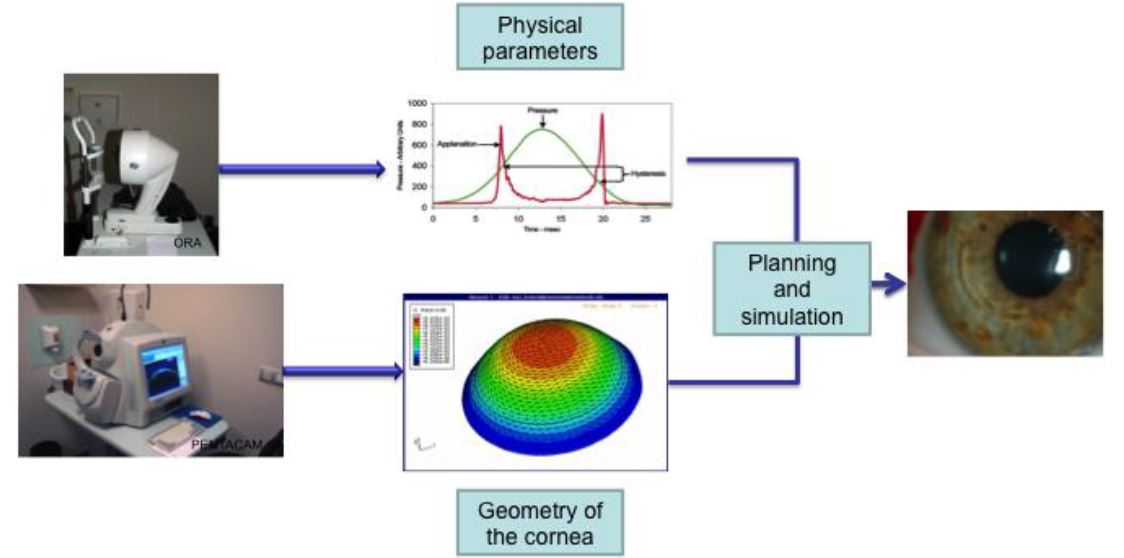
\includegraphics[scale=0.9]{img.png}
\end{center}

Tomamos la siguiente base de datos relativa a la clasificación de planetas extrasolares como habitables o no. Para ello disponemos de tres variables predictivas: Tamaño, Órbita y Temperatura. La variable clase (Habitable) es binaria {sí, no}. Nótese que la columna “Contador” no es una variable predictiva, si no que nos sirve para mostrar de forma “comprimida” la base de datos, indicándose cuantas instancias existen para cada una de las configuraciones mostradas. Así, podemos ver que nuestra base de datos tiene 800 instancias, y no 8 como correspondería al número de filas de la tabla.

\begin{questions}
	
% Pregunta 1
{\bf \question Construye un clasificador Naive Bayes para la tabla suministrada. Debes detallar todas las tablas de probabilidad.}

Para este entregable, primero he preparado un fichero de datos CSV ("dataset.csv"), a partir de la tabla proporcionada, usando el lenguaje de programación Python, donde el fichero CSV resultante contiene las 800 instancias.

A continuación se puede observar el código en Python utilizado,

\newpage

\lstset{
	language=Python,
	literate={ñ}{{\~n}}1
	{Ó}{{\'O}}1
}
\begin{lstlisting}[basicstyle=\small, tabsize=2]
import csv
import pandas as pd

data = {
	"Contador": [170, 20, 45, 139, 30, 130, 255, 11],
	"Tamaño": ["Grande", "Grande", "Pequeño", "Pequeño", "Grande", 
		"Grande", "Pequeño", "Pequeño"],
	"Órbita": ["Cercana", "Cercana", "Lejana", "Cercana", "Lejana", 
		"Cercana", "Lejana", "Cercana"],
	"Temperatura": ["M", "A", "M", "M", "B", "B", "B", "A"],
	"Habitable": ["Si", "Si", "Si", "Si", "No", "No", "No", "No"]
}

df = pd.DataFrame(data, columns=list(data.keys()))
columnames = df.columns.tolist()
contador = data["Contador"]

with open("dataset.csv", "w") as fd:
	csv.writer(fd).writerow(columnames)  # add column names
	for n in range(len(contador)):
		for i in range(contador[n]):
			df.loc[[n]].to_csv(fd, index=False, header=False, mode="a")
\end{lstlisting}

Después he transformado el conjunto de datos para eliminar la variable Contador, ya que no es una variable predictiva.

A continuación se puede observar el código en Python añadido,

\begin{lstlisting}[language=Python, basicstyle=\small, tabsize=2]
df = pd.read_csv('dataset.csv')
df = df.drop(["Contador"], axis=1)
df.to_csv('dataset.csv', index=False)
\end{lstlisting}

Finalmente, he utilizado el software \href{https://www.knime.com/}{KNIME} para la construcción del clasificador Naive Bayes para el conjunto de datos. Concretamente, el clasificador crea un modelo bayesiano a partir de los datos. Calcula el número de filas por valor de atributo por clase para atributos nominales y la distribución gaussiana para atributos numéricos. 

Si usamos Naive Bayes Learner, 

\begin{center}
	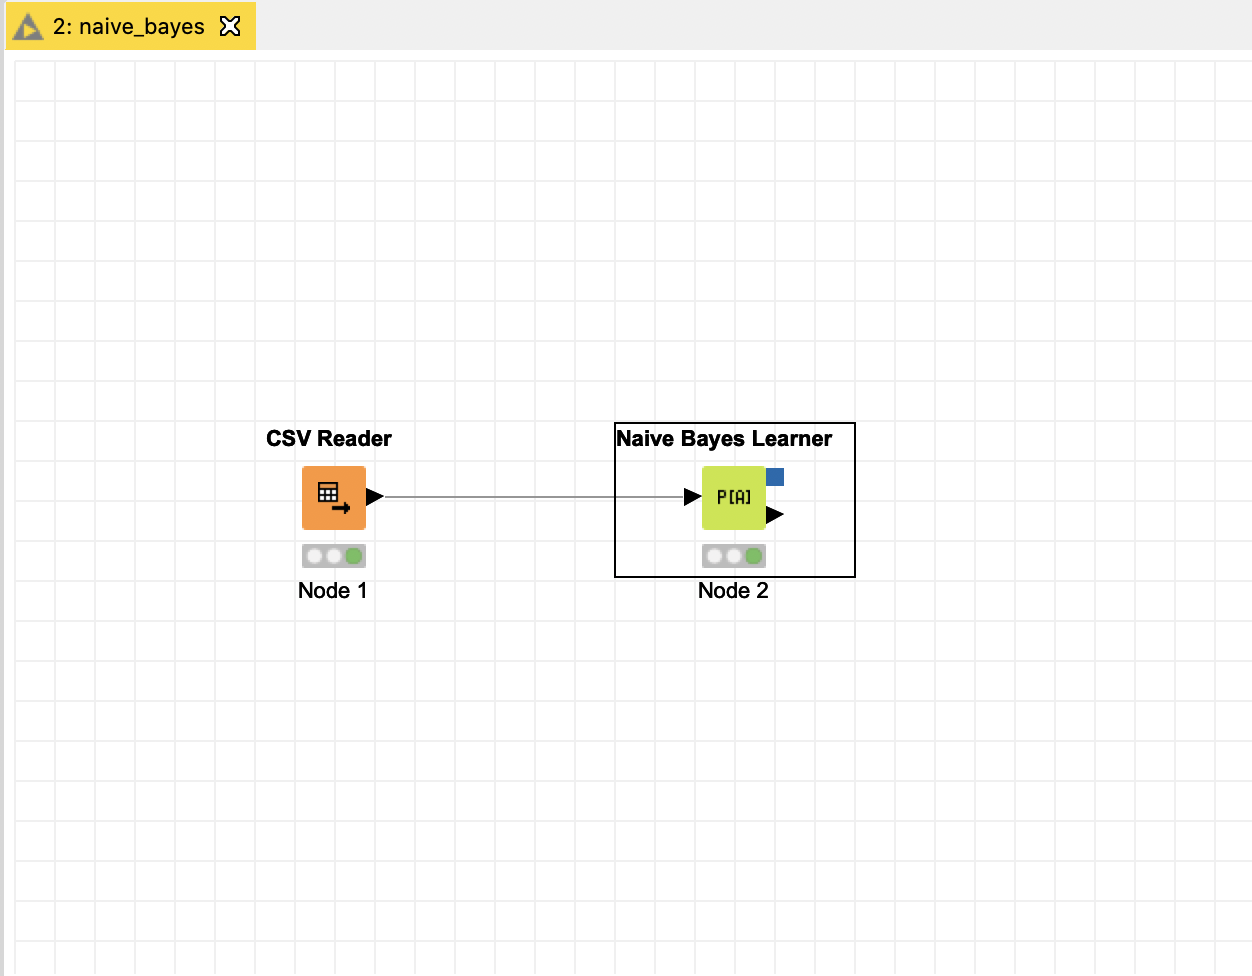
\includegraphics[scale=0.35]{workflow.png}
\end{center}

Por ejemplo, podemos obtener información como:

\begin{center}
	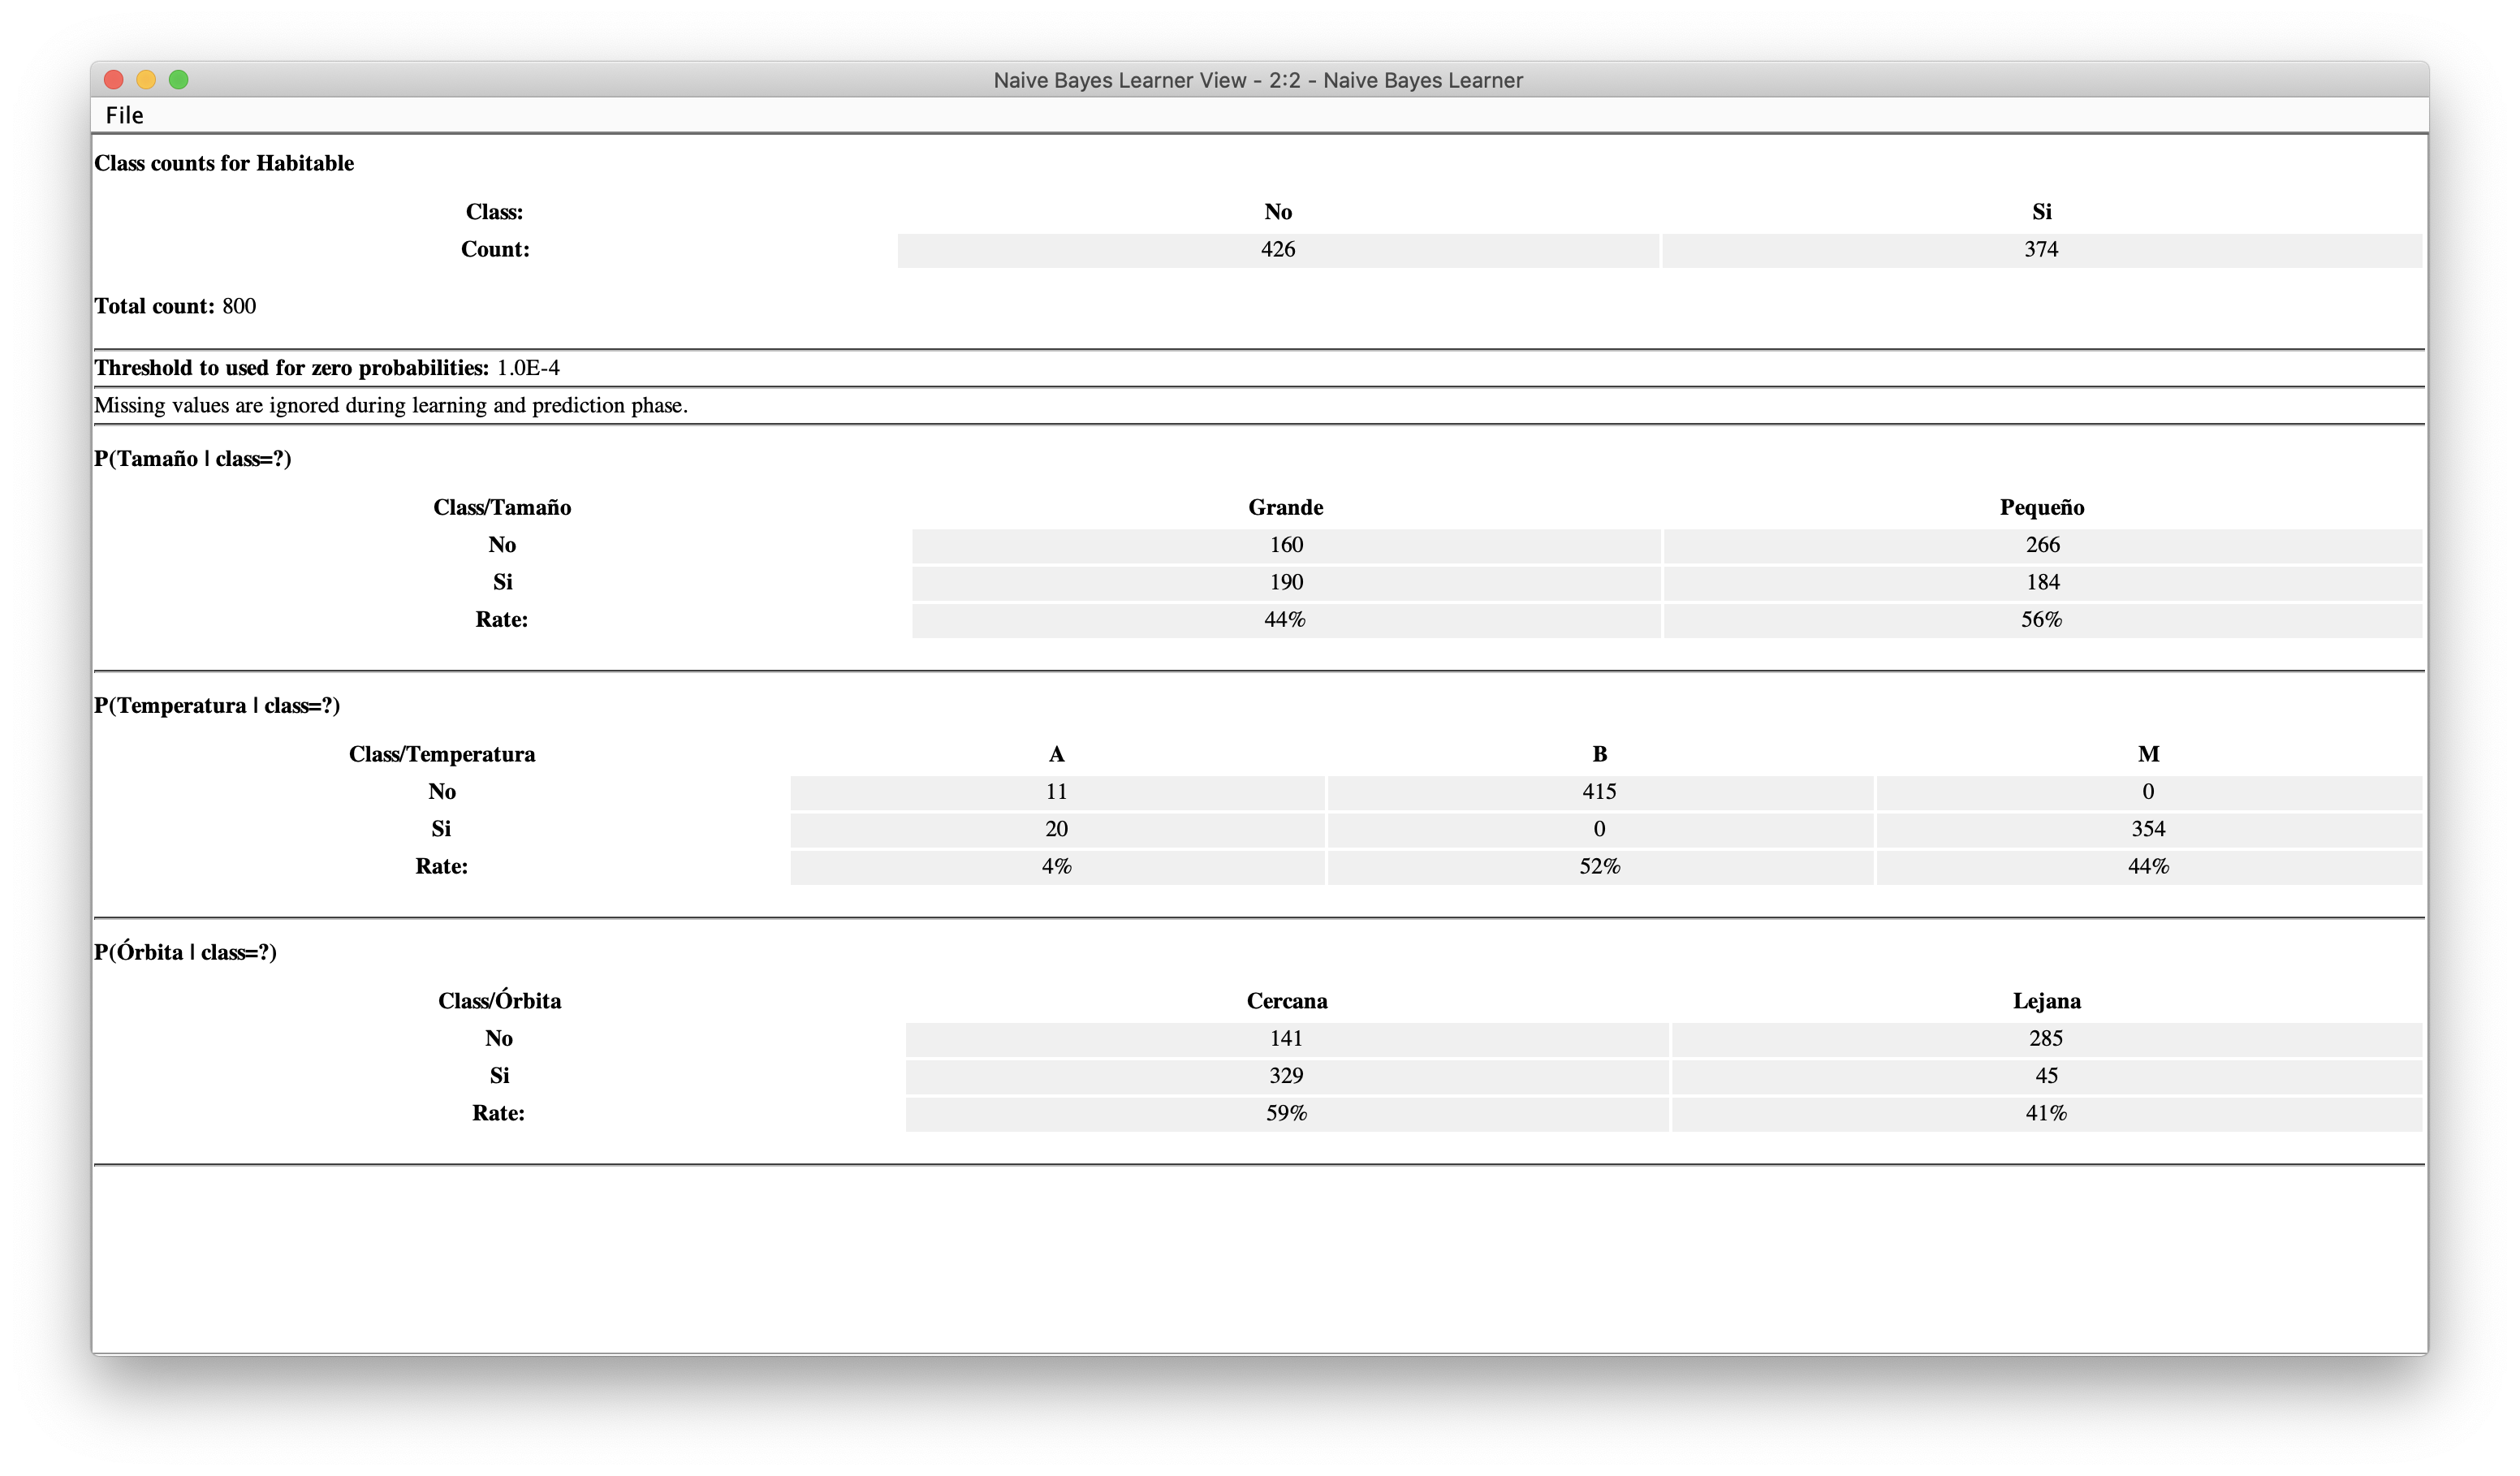
\includegraphics[scale=0.3]{table.png}
\end{center}

KNIME además, és un software que podría detallar automáticamente las tablas de probabilidad. Pero para esta actividad he preferido hacer las tablas de probabilidad manualmente como aprendizaje.

\section*{Tablas de probabilidad}

P(Habitable=Sí) = (374+1)/(800+2) = 0.467

P(Habitable=No) = (426+1)/(800+2) = 0.532

\begin{center}
	\begin{tabular}{ |c|c|c| } 
		\hline
		P(Habitable) & Habitable = Sí & Habitable = No \\
		\hline
		& 0.467 & 0.532 \\ 
		\hline
	\end{tabular}
\end{center}

P(Tamaño=Grande$|$Habitable=Sí) = (190+1)/(800+2) = 0.238

P(Tamaño=Grande$|$Habitable=No) = (160+1)/(800+2) = 0.201

P(Tamaño=Pequeña$|$Habitable=Sí) = (184+1)/(800+2) = 0.231

P(Tamaño=Pequeña$|$Habitable=No) = (266+1)/(800+2) = 0.333

\begin{center}
	\begin{tabular}{ |c|c|c| } 
		\hline
		P(Tamaño$|$Habitable) & Habitable = Sí & Habitable = No \\
		\hline
		Tamaño = Grande & 0.238 & 0.201 \\ 
		\hline
		Tamaño = Pequeña & 0.231 & 0.333 \\ 
		\hline
	\end{tabular}
\end{center}

P(Órbita=Cercana$|$Habitable=Sí) = (329+1)/(800+2) = 0.411

P(Órbita=Cercana$|$Habitable=No) = (141+1)/(800+2) = 0.177

P(Órbita=Lejana$|$Habitable=Sí) = (45+1)/(800+2) = 0.057

P(Órbita=Lejana$|$Habitable=No) = (285+1)/(800+2) = 0.357

\begin{center}
	\begin{tabular}{ |c|c|c| } 
		\hline
		P(Órbita$|$Habitable) & Habitable = Sí & Habitable = No \\
		\hline
		Órbita = Cercana & 0.411 & 0.177 \\ 
		\hline
		Órbita = Lejana & 0.057 & 0.357 \\ 
		\hline
	\end{tabular}
\end{center}

P(Temperatura=A$|$Habitable=Sí) = (20+1)/(800+2) = 0.026

P(Temperatura=A$|$Habitable=No) = (11+1)/(800+2) = 0.015

P(Temperatura=B$|$Habitable=Sí) = (0+1)/(800+2) = 1.25x10$^-3$

P(Temperatura=B$|$Habitable=No) = (415+1)/(800+2) = 0.519

P(Temperatura=M$|$Habitable=Sí) = (354+1)/(800+2) = 0.445

P(Temperatura=M$|$Habitable=No) = (0+1)/(800+2) = 1.25x10$^-3$

\begin{center}
	\begin{tabular}{ |c|c|c| } 
		\hline
		P(Temperatura$|$Habitable) & Habitable = Sí & Habitable = No \\
		\hline
		Temperatura = A & 0.026 & 0.015 \\ 
		\hline
		Temperatura = B & 1.25x10$^-3$ & 0.519 \\ 
		\hline
		Temperatura = M & 0.445 & 1.25x10$^-3$ \\ 
		\hline
	\end{tabular}
\end{center}

% Pregunta 2
{\bf \question ¿Cuántos parámetros necesita tu clasificador? ¿Cuántos necesitaría para especificar la distribución de probabilidad conjunta (DPC)?}

Dado n = 800, como el numero total de instancias de la base de datos, el clasificador Naive Bayes necesita n parámetros. Y para especificar DPC se necesitarían 2$^n$ parámetros.

% Pregunta 3
{{\bf \question Clasifica los siguientes registros y muestra la distribución de probabilidad resultante:}
	
Volviendo a utilizar la corrección de Laplace,

\begin{enumerate}
	{\bf \item (Tamaño=Grande, Órbita=Cercana, Temperatura=M)}
	
	Se estima para las dos etiquetas de la variable clase Habitable (Sí, No): 
	
	\begin{itemize}
		\item P(Sí)*P(Tamaño=Grande$|$Sí)*P(Órbita=Cercana$|$Sí)*P(Temperatura=M$|$Sí) = 0.467 * 0.238 * 0.411 * 0.445 = 0.020 
		
		\item P(No)*P(Tamaño=Grande$|$No)*P(Órbita=Cercana$|$No)*P(Temperatura=M$|$No) = 0.532 * 0.201 * 0.177 * 1.25x10$^-3$ = 2.36x10$^-5$

		\item P(Tamaño=Grande, Órbita=Cercana, Temperatura=M) = 0.020 + 2.36x10$^-5$ = 0.0200236
		
	\end{itemize}
	
	{\bf \item (Tamaño=Grande, Órbita=Lejana, Temperatura=A)}
	
	Se vuelve a estimar para las dos etiquetas de la variable clase Habitable (Sí, No): 
	
	\begin{itemize}
		\item P(Sí)*P(Tamaño=Grande$|$Sí)*P(Órbita=Lejana$|$Sí)*P(Temperatura=A$|$Sí) = 0.467 * 0.238 * 0.057 * 0.026 = 1.65x10$^-4$ 
		
		\item P(No)*P(Tamaño=Grande$|$No)*P(Órbita=Lejana$|$No)*P(Temperatura=A$|$No) = 0.532 * 0.201 * 0.357 * 0.015 = 5.73x10$^-4$
		
		\item P(Tamaño=Grande, Órbita=Lejana, Temperatura=A) = 1.65x10$^-4$ + 5.73x10$^-4$ = 7.38x10$^-4$
	\end{itemize}
\end{enumerate}
}

% Pregunta 4
{\bf \question Si usáramos la DPC como clasificador y para todo registro obtuviéramos el mismo resultado que usando el clasificador Naive Bayes, ¿qué conclusión obtendríamos?}

Que en la base de datos utilizada hay muchas variables y que pocas de ellas son relevantes.

\end{questions}

\end{document}